% Options for packages loaded elsewhere
% Options for packages loaded elsewhere
\PassOptionsToPackage{unicode}{hyperref}
\PassOptionsToPackage{hyphens}{url}
\PassOptionsToPackage{dvipsnames,svgnames,x11names}{xcolor}
%
\documentclass[
  british,
  a4paper,
]{article}
\usepackage{xcolor}
\usepackage{amsmath,amssymb}
\setcounter{secnumdepth}{-\maxdimen} % remove section numbering
\usepackage{iftex}
\ifPDFTeX
  \usepackage[T1]{fontenc}
  \usepackage[utf8]{inputenc}
  \usepackage{textcomp} % provide euro and other symbols
\else % if luatex or xetex
  \usepackage{unicode-math} % this also loads fontspec
  \defaultfontfeatures{Scale=MatchLowercase}
  \defaultfontfeatures[\rmfamily]{Ligatures=TeX,Scale=1}
\fi
\usepackage{lmodern}
\ifPDFTeX\else
  % xetex/luatex font selection
\fi
% Use upquote if available, for straight quotes in verbatim environments
\IfFileExists{upquote.sty}{\usepackage{upquote}}{}
\IfFileExists{microtype.sty}{% use microtype if available
  \usepackage[]{microtype}
  \UseMicrotypeSet[protrusion]{basicmath} % disable protrusion for tt fonts
}{}
\makeatletter
\@ifundefined{KOMAClassName}{% if non-KOMA class
  \IfFileExists{parskip.sty}{%
    \usepackage{parskip}
  }{% else
    \setlength{\parindent}{0pt}
    \setlength{\parskip}{6pt plus 2pt minus 1pt}}
}{% if KOMA class
  \KOMAoptions{parskip=half}}
\makeatother
% Make \paragraph and \subparagraph free-standing
\makeatletter
\ifx\paragraph\undefined\else
  \let\oldparagraph\paragraph
  \renewcommand{\paragraph}{
    \@ifstar
      \xxxParagraphStar
      \xxxParagraphNoStar
  }
  \newcommand{\xxxParagraphStar}[1]{\oldparagraph*{#1}\mbox{}}
  \newcommand{\xxxParagraphNoStar}[1]{\oldparagraph{#1}\mbox{}}
\fi
\ifx\subparagraph\undefined\else
  \let\oldsubparagraph\subparagraph
  \renewcommand{\subparagraph}{
    \@ifstar
      \xxxSubParagraphStar
      \xxxSubParagraphNoStar
  }
  \newcommand{\xxxSubParagraphStar}[1]{\oldsubparagraph*{#1}\mbox{}}
  \newcommand{\xxxSubParagraphNoStar}[1]{\oldsubparagraph{#1}\mbox{}}
\fi
\makeatother


\usepackage{longtable,booktabs,array}
\newcounter{none} % for unnumbered tables
\usepackage{calc} % for calculating minipage widths
% Correct order of tables after \paragraph or \subparagraph
\usepackage{etoolbox}
\makeatletter
\patchcmd\longtable{\par}{\if@noskipsec\mbox{}\fi\par}{}{}
\makeatother
% Allow footnotes in longtable head/foot
\IfFileExists{footnotehyper.sty}{\usepackage{footnotehyper}}{\usepackage{footnote}}
\makesavenoteenv{longtable}
\usepackage{graphicx}
\makeatletter
\newsavebox\pandoc@box
\newcommand*\pandocbounded[1]{% scales image to fit in text height/width
  \sbox\pandoc@box{#1}%
  \Gscale@div\@tempa{\textheight}{\dimexpr\ht\pandoc@box+\dp\pandoc@box\relax}%
  \Gscale@div\@tempb{\linewidth}{\wd\pandoc@box}%
  \ifdim\@tempb\p@<\@tempa\p@\let\@tempa\@tempb\fi% select the smaller of both
  \ifdim\@tempa\p@<\p@\scalebox{\@tempa}{\usebox\pandoc@box}%
  \else\usebox{\pandoc@box}%
  \fi%
}
% Set default figure placement to htbp
\def\fps@figure{htbp}
\makeatother



\ifLuaTeX
\usepackage[bidi=basic,shorthands=off]{babel}
\else
\usepackage[bidi=default,shorthands=off]{babel}
\fi
\ifLuaTeX
  \usepackage{selnolig} % disable illegal ligatures
\fi


\setlength{\emergencystretch}{3em} % prevent overfull lines

\providecommand{\tightlist}{%
  \setlength{\itemsep}{0pt}\setlength{\parskip}{0pt}}



 


\makeatletter
\@ifpackageloaded{tcolorbox}{}{\usepackage[skins,breakable]{tcolorbox}}
\@ifpackageloaded{fontawesome5}{}{\usepackage{fontawesome5}}
\definecolor{quarto-callout-color}{HTML}{909090}
\definecolor{quarto-callout-note-color}{HTML}{0758E5}
\definecolor{quarto-callout-important-color}{HTML}{CC1914}
\definecolor{quarto-callout-warning-color}{HTML}{EB9113}
\definecolor{quarto-callout-tip-color}{HTML}{00A047}
\definecolor{quarto-callout-caution-color}{HTML}{FC5300}
\definecolor{quarto-callout-color-frame}{HTML}{acacac}
\definecolor{quarto-callout-note-color-frame}{HTML}{4582ec}
\definecolor{quarto-callout-important-color-frame}{HTML}{d9534f}
\definecolor{quarto-callout-warning-color-frame}{HTML}{f0ad4e}
\definecolor{quarto-callout-tip-color-frame}{HTML}{02b875}
\definecolor{quarto-callout-caution-color-frame}{HTML}{fd7e14}
\makeatother
\makeatletter
\@ifpackageloaded{caption}{}{\usepackage{caption}}
\AtBeginDocument{%
\ifdefined\contentsname
  \renewcommand*\contentsname{Table of contents}
\else
  \newcommand\contentsname{Table of contents}
\fi
\ifdefined\listfigurename
  \renewcommand*\listfigurename{List of Figures}
\else
  \newcommand\listfigurename{List of Figures}
\fi
\ifdefined\listtablename
  \renewcommand*\listtablename{List of Tables}
\else
  \newcommand\listtablename{List of Tables}
\fi
\ifdefined\figurename
  \renewcommand*\figurename{Figure}
\else
  \newcommand\figurename{Figure}
\fi
\ifdefined\tablename
  \renewcommand*\tablename{Table}
\else
  \newcommand\tablename{Table}
\fi
}
\@ifpackageloaded{float}{}{\usepackage{float}}
\floatstyle{ruled}
\@ifundefined{c@chapter}{\newfloat{codelisting}{h}{lop}}{\newfloat{codelisting}{h}{lop}[chapter]}
\floatname{codelisting}{Listing}
\newcommand*\listoflistings{\listof{codelisting}{List of Listings}}
\makeatother
\makeatletter
\makeatother
\makeatletter
\@ifpackageloaded{caption}{}{\usepackage{caption}}
\@ifpackageloaded{subcaption}{}{\usepackage{subcaption}}
\makeatother
\usepackage{bookmark}
\IfFileExists{xurl.sty}{\usepackage{xurl}}{} % add URL line breaks if available
\urlstyle{same}
% fallback for those not using the hyperref driver hyperxmp:
\makeatletter
\@ifundefined{xmpquote}{\newcommand{\xmpquote}[1]{#1}}{}
\makeatother
\hypersetup{
  pdftitle={A quarterly panel of every English local authority},
  pdfauthor={Carlos Galindo},
  pdflang={en-GB},
  colorlinks=true,
  linkcolor={blue},
  filecolor={Maroon},
  citecolor={Blue},
  urlcolor={Blue},
  pdfcreator={LaTeX via pandoc}}


\title{A quarterly panel of every English local authority}
\usepackage{etoolbox}
\makeatletter
\providecommand{\subtitle}[1]{% add subtitle to \maketitle
  \apptocmd{\@title}{\par {\large #1 \par}}{}{}
}
\makeatother
\subtitle{One consistent dataset for testing what housing benefit and
the 2021--24 rate rises did to private rents}
\author{Carlos Galindo}
\date{}
\begin{document}
\maketitle


\begin{tcolorbox}[enhanced jigsaw, arc=.35mm, bottomrule=.15mm, breakable, colback=white, colframe=quarto-callout-note-color-frame, left=2mm, leftrule=.75mm, opacityback=0, rightrule=.15mm, toprule=.15mm]

\vspace{-3mm}\textbf{At a glance}\vspace{3mm}

\begin{itemize}
\tightlist
\item
  \textbf{Question.} Did higher interest rates raise private rents, and
  did housing benefit end up in landlords' pockets rather than tenants'
  budgets?
\item
  \textbf{Approach.} A quarterly panel of all 290 English local
  authorities, 2019 to early 2024, built from official housing, benefit
  and labour-market statistics, so that areas can be compared with each
  other within the same region and quarter.
\item
  \textbf{Finding.} Rents rose no faster where landlords were more
  exposed to higher interest rates, and the design rules out roughly
  four-fifths of full pass-through. Where more tenants relied on housing
  benefit, rent growth slowed once the allowance was frozen: negative in
  all 23 specifications, and clearly so in the better-powered window.
\item
  \textbf{Why it matters.} Local rent growth is driven by many things at
  once. A panel that absorbs what areas share is what lets a policy
  effect be told apart from the noise.
\end{itemize}

\end{tcolorbox}

\subsection{The question}\label{the-question}

Between 2021 and 2024 the Bank of England raised its policy rate from
0.1\% to 5.25\%. Over the same years private rents rose fast, and a
frequent claim in the policy debate was that landlords were simply
passing higher mortgage costs on to tenants. Over the same years the
cash value of housing support for private renters (the Local Housing
Allowance) was frozen, then partly restored, then frozen again. Both
stories matter for policy, and both are hard to test with national
totals: rents, rates, inflation and benefit policy all move together in
time, so a single national series cannot say which one is doing the
work.

Areas, however, differ. They differ in how expensive housing is relative
to rents, and in how many tenants depend on benefit. If a policy or a
shock acts through one of those differences, rents should respond
differently in the areas that have more of it. That is the logic of a
quasi-experiment, and it needs one thing before anything else: a clean,
comparable, quarterly dataset covering every authority, over a window
that includes the events of interest. This project built that dataset
and used it for two studies.

\subsection{Approach}\label{approach}

\subsubsection{The panel}\label{the-panel}

The panel covers all 290 local authorities in England, quarterly, from
the first quarter of 2019 to the first quarter of 2024. That is 21
quarters and 6,090 authority-quarter observations in the headline
sample. It combines three kinds of official statistics:

\begin{itemize}
\tightlist
\item
  \textbf{Housing.} Median private rents for two-bedroom homes, house
  prices, and the rental-market areas used to set benefit rates.
\item
  \textbf{Benefits.} Housing benefit and Universal Credit caseloads in
  the private rented sector, expressed as a share of the private rental
  stock. This is ``benefit intensity''.
\item
  \textbf{Labour market.} The claimant count and the 10th-percentile
  wage, used as time-varying controls. The low-paid wage is the relevant
  outside option for the tenants who depend on benefit.
\end{itemize}

Most of the work is unglamorous and decisive. Boundaries change, so
every source had to be mapped to a single set of authority codes. Rents
are published on a different geography from the one on which benefits
are administered, so a crosswalk was needed. The official private-rent
series changed methodology during the window, so the analysis window was
locked at early 2024 rather than splicing across the break, and an
extension is treated as optional until an overlap check has been done.
The set of 290 authorities was locked once, so both studies use the same
sample.

\subsubsection{Two predetermined
exposures}\label{two-predetermined-exposures}

The key design choice is to measure how exposed an area is \emph{before}
the events, so that exposure cannot respond to them.

\begin{itemize}
\tightlist
\item
  \textbf{Interest sensitivity.} The 2019 ratio of average house price
  to annual rent, standardised across authorities. Where prices are high
  relative to rents, a given rise in financing cost eats a larger share
  of rental income, so a landlord restoring a target yield would have to
  raise rents by more. Under full cost-plus pass-through the required
  percentage rent rise is proportional to this ratio.
\item
  \textbf{Benefit intensity.} The pre-period share of private rented
  homes with a benefit claimant. It averages 4.4\% across authorities
  and exceeds 8\% in the top decile, concentrated in coastal towns,
  post-industrial districts and a few inner-London boroughs.
\end{itemize}

\subsubsection{The estimating design}\label{the-estimating-design}

Both studies use the same skeleton. The outcome is year-on-year rent
growth. The regressor of interest is the exposure interacted with the
event: the change in the rate for the first study, the 2021 benefit
re-freeze for the second. Authority fixed effects remove each area's own
average growth, and region-by-quarter fixed effects remove everything
common to a region in a given quarter, including every nationwide shock.
What is left is the question that matters: among authorities in the same
region and quarter, did the more exposed ones diverge as the event
unfolded? Standard errors are clustered by authority.

For the rate study the treatment is not Bank Rate but the effective rate
on the \emph{outstanding} stock of mortgages, which is what landlords
with existing fixed-term debt actually pay. It rose far more slowly,
from about 2.05\% in 2021 to about 3.8\% by early 2024. The
specification, its placebo window and a distributed-lag variant were
fixed before any estimation on real data.

\begin{figure}

\centering{

\pandocbounded{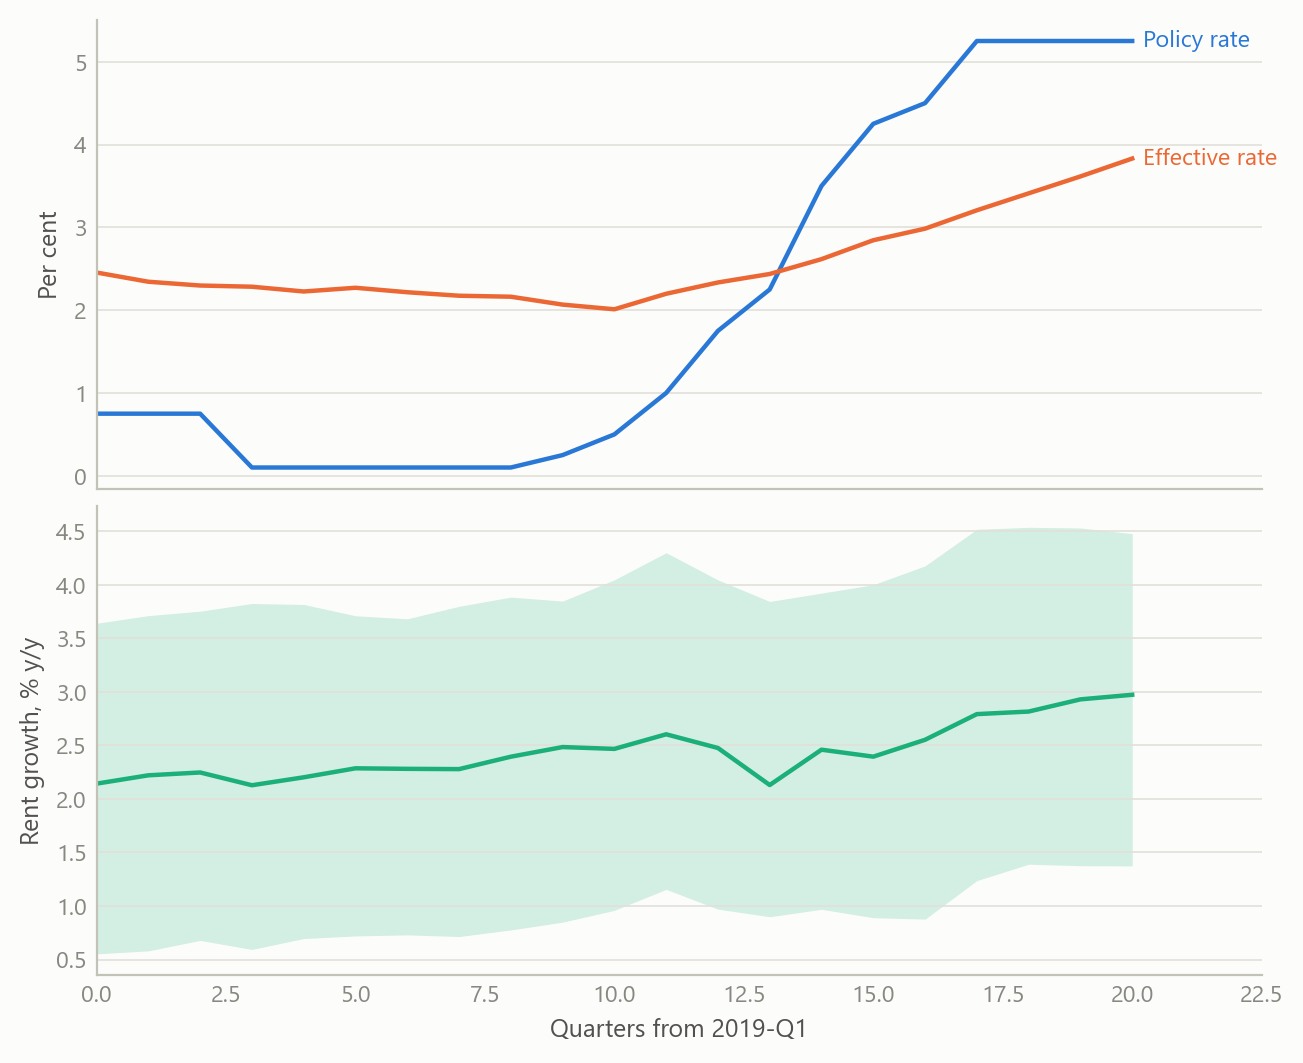
\includegraphics[keepaspectratio]{index_files/figure-latex/fig-panel-output-1.png}}

}

\caption{\label{fig-panel}The two series the design compares, and the
spread it exploits (simulated data). Top: policy rate and effective
mortgage-stock rate. Bottom: year-on-year rent growth across 290
authorities, median with 10th to 90th percentile band.}

\end{figure}%

\subsection{What the work shows}\label{what-the-work-shows}

\subsubsection{Rate pass-through: a bounded
null}\label{rate-pass-through-a-bounded-null}

The central estimate for the rate study is essentially zero. The
interaction coefficient is −0.00013 with a p-value of 0.9835: more
interest-sensitive areas did not see faster rent growth as financing
costs rose. A null only matters if it excludes something, so the study
calibrates what it excludes. The largest differential effect the design
could plausibly have missed is about 0.59\% of cumulative rent growth
per standard deviation of interest sensitivity, while full cost-plus
pass-through, over a range of plausible loan-to-value ratios, mortgaged
shares and a tax amplifier for individual landlords, would require 2.8\%
to 5.0\%. The data therefore rule out roughly four-fifths of
frictionless pass-through through this channel.

Two checks make the null credible rather than empty. First, results are
uniformly small and insignificant across alternative rate measures,
transformations, lag structures and samples. Second, a raw cross-section
tells a seemingly opposite story: more interest-sensitive areas had
\emph{slower} rent growth over the cycle. A true pre-period with a flat
policy rate shows the same gradient, and a steeper one (0.01328 before,
0.00887 during, both negative). It is a long-running convergence of
cheaper areas catching up, not a monetary effect, and it is exactly what
the authority fixed effects absorb. One placebo window did fail, and the
work reports it with its diagnosed cause, the 2020--21 pandemic
reshuffling of London and the South East, rather than dropping it.

\begin{figure}

\centering{

\pandocbounded{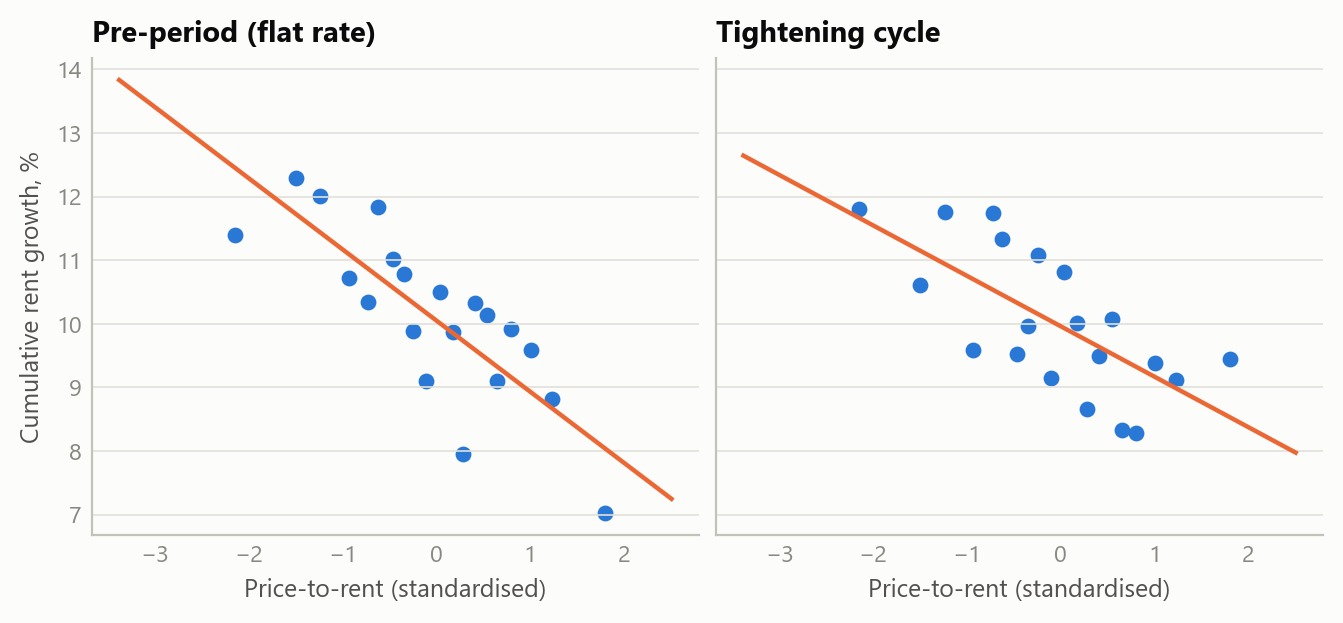
\includegraphics[keepaspectratio]{index_files/figure-latex/fig-pretrend-output-1.png}}

}

\caption{\label{fig-pretrend}Why a panel and not a cross-section
(simulated data). In both a flat-rate pre-period and the tightening
cycle, areas with higher price-to-rent grew rents more slowly. The
gradient predates the rate rises, so it cannot be a rate effect.}

\end{figure}%

\subsubsection{Benefit incidence: a consistent
direction}\label{benefit-incidence-a-consistent-direction}

The second study treats the benefit freeze as a natural experiment.
Housing support is meant to reach the 30th percentile of local rents. It
is reset to that level at each uplift and then held in cash terms, so
during the 2021--24 re-freeze it fell steadily behind a market whose
lower tail was growing at close to five per cent a year. If the
allowance acts as a floor under rents in the benefit-dependent part of
the market, areas with more claimants should see rent growth \emph{slow}
once the floor stopped rising. The 2020 uplift is the mirror-image test,
but it landed in a soft pandemic market and is a weak one.

Across 23 specifications varying the window, spatial controls, bedroom
mix and treatment of outliers, every estimate of the re-freeze effect is
negative, with no sign reversals. The specifications share one
cross-section, so this reads as robustness of the sign, not as 23
independent tests. The baseline estimate is small and imprecise
(−0.0174, p = 0.142), which is the expected signature when sitting
tenants and reluctance to cut rents bias the estimate towards zero. The
better-powered window, which uses the uplift period as the baseline,
gives −0.0498 (p = 0.0033). Excluding the top decile of authorities by
net in-migration leaves the sign unchanged, so the pattern is not just
people moving.

\begin{figure}

\centering{

\pandocbounded{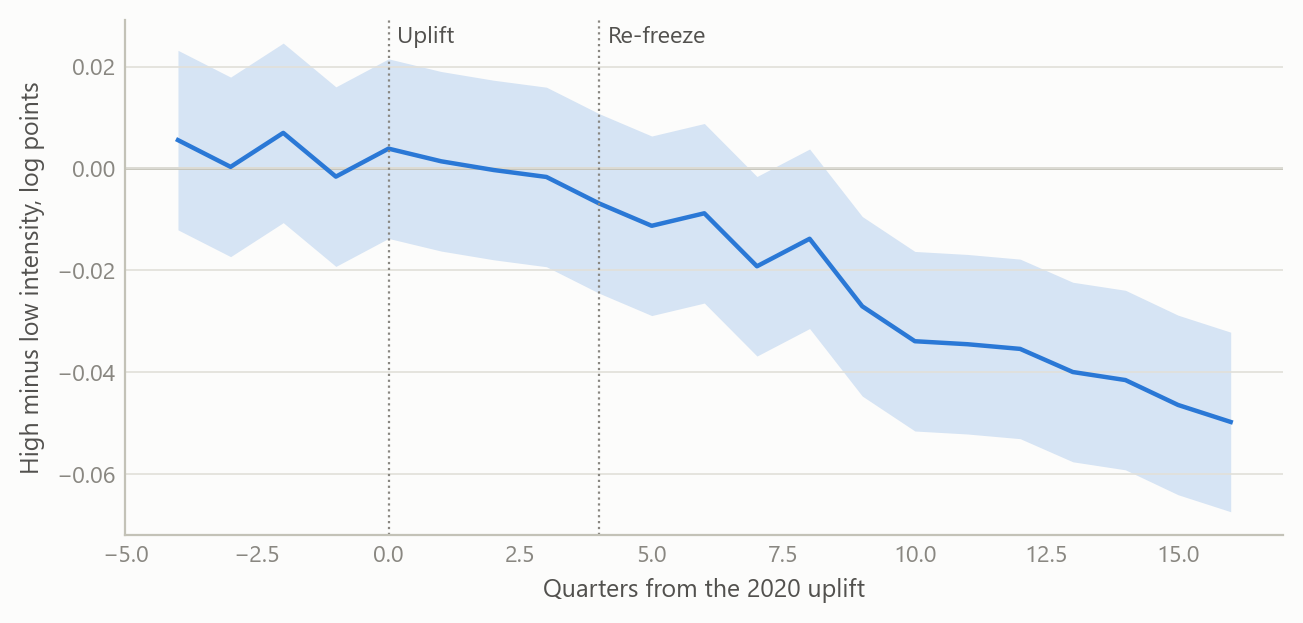
\includegraphics[keepaspectratio]{index_files/figure-latex/fig-event-output-1.png}}

}

\caption{\label{fig-event}The shape of an event-study on benefit
intensity (simulated data). Differential rent growth of high- relative
to low-intensity authorities, with the uplift and the re-freeze marked.
Simulated to illustrate the design, not the estimates.}

\end{figure}%

\subsection{Insights}\label{insights}

\begin{enumerate}
\def\labelenumi{\arabic{enumi}.}
\tightlist
\item
  \textbf{Exposure must be fixed before the event.} Both studies use
  2018--19 values, so an area's position cannot be a response to the
  rate path or the freeze. Most of the credibility is bought there, at
  no cost in data.
\item
  \textbf{A null needs a yardstick.} ``No significant effect'' says
  little. Converting it to economic units and comparing it with what the
  theory predicts turns it into a statement about what has been
  excluded.
\item
  \textbf{Show the confound before the reader does.} The negative
  cross-sectional gradient looks like a perverse channel until a
  pre-period shows it was already there. Putting that in the paper turns
  the strongest objection into the best argument for the design.
\item
  \textbf{Treat the treatment variable as a finding.} Policy rates and
  the rate landlords actually pay diverged for years. Choosing the wrong
  one would have overstated the shock.
\item
  \textbf{Read two results together.} Rate pass-through through
  landlords' financing costs looks small, while the frozen benefit floor
  appears to bind. Together they suggest the pressure sat on the tenant
  side of the market, and that monetary and fiscal policy were pulling
  in different directions.
\end{enumerate}

\subsection{Limits and next steps}\label{limits-and-next-steps}

An area panel cannot see what happens inside an area. A cost shock that
passes through hardest where tenant demand is least elastic, or a
landlord with a portfolio across authorities, is below its resolution.
The null is silent on those mechanisms rather than exculpatory, and a
household- or landlord-level incidence design is the right next test.

The window is also short and mid-transmission. The effective mortgage
rate had only reached about 3.8\% by early 2024, and fixed-rate deals
taken out in 2021--22 were still rolling off. Tenancies reprice at
renewal, and the rent series records rents currently paid, so adjustment
is staggered and slow by construction. The rate study therefore commits
to a replication once transmission is complete. Finally, the benefit
estimates identify the direction of the effect robustly but their size
depends on the specification, and the sustenance reading of housing
support that sits alongside them is consistent with the results without
being tested by them.

\subsection{About the evidence}\label{about-the-evidence}

The panel and both studies are real: 290 authorities, 21 quarters,
official statistics, built between 2024 and 2026 during a period of
independent research. The figures here are simulated from the same
structure (authorities, quarters, exposures, event timing) and
illustrate the design only. The estimates in the text are the project's
own results.

Figures and tables marked \emph{simulated} are generated from simulated
data built to share the structure of the analysis (its variables,
horizons and frequencies). They show how the method works and what its
output looks like; they are not the project's results. Results stated in
the text are the project's own. Methods are described at the level of a
methods section. Code and data pipelines are not reproduced here.




\end{document}
